% !TeX program = xelatex
% UTF-8; compile with XeLaTeX twice from this directory.
\documentclass[a4paper,11pt]{article}
\usepackage[english]{babel}
\usepackage[T1]{fontenc}
\usepackage{lmodern}
\usepackage[margin=2.35cm,headheight=14pt]{geometry}
\usepackage{amsmath,amssymb,bm,booktabs,tabularx,array}
\usepackage{graphicx,float,caption,enumitem,xcolor,fancyhdr}
\usepackage[numbers,sort&compress]{natbib}
\usepackage{hyperref,xurl,microtype}
\usepackage[section]{placeins}
\usepackage{needspace}
\definecolor{navy}{HTML}{17324D}
\definecolor{teal}{HTML}{287D8E}
\hypersetup{colorlinks=true,linkcolor=navy,citecolor=teal,urlcolor=teal,
 pdftitle={Auto-ORCA: An LLM-Guided Agent for Autonomous DFT Calculations},
 pdfauthor={CHEN GENG},pdflang={en}}
\urlstyle{same}
\graphicspath{{figures/}}
\renewcommand{\arraystretch}{1.18}
\setlength{\tabcolsep}{5pt}
\setlength{\emergencystretch}{3em}
\clubpenalty=10000
\widowpenalty=10000
\linespread{1.08}
\renewcommand{\topfraction}{0.9}
\renewcommand{\bottomfraction}{0.85}
\renewcommand{\textfraction}{0.08}
\renewcommand{\floatpagefraction}{0.8}
\setlist{nosep,leftmargin=2em}
\captionsetup{font=small,labelfont=bf,labelsep=period}
\pagestyle{fancy}
\fancyhf{}
\fancyhead[L]{\small Auto-ORCA}
\fancyfoot[C]{\thepage}
\newcolumntype{Y}{>{\raggedright\arraybackslash}X}
\newcommand{\Eh}{E_{\mathrm h}}
\newcommand{\code}[1]{\texttt{#1}}
\title{\vspace{-1.0cm}\LARGE\bfseries
 Auto-ORCA: An LLM-Guided Agent\\[0.2em]
 for Autonomous DFT Calculations}
\author{\large CHEN GENG}
\date{}
\begin{document}
\maketitle
\vspace{-0.7cm}
\begin{abstract}
  Molecular density functional theory (DFT) studies require the coordination of structure preparation, electronic-structure calculations, result assessment, and subsequent calculations.
  This work presents Auto-ORCA, which connects the task-planning and code-generation capabilities of large language models to a managed ORCA execution environment.
  Calculations are performed through a unified ORCA entry point, and their outputs inform plan revisions.
  The system stores scientific objectives separately from execution plans, retrieves versioned domain information as needed, and records the relationships between results, inputs, geometries, and raw outputs.
  Seven test cases examine geometry optimization and vibrational frequencies, candidate conformer energies, dihedral scans, vertical excitations, environmental effects, and response tensors.
  When success is assessed by the production of computational outputs for each test problem, the success rate is $6/7$.
  Ethanol optimization converged and yielded 21 positive frequencies and no imaginary frequencies; single-point energies were compared for six candidate geometries of \textit{n}-hexane; five singlet excitation energies were obtained for acetone; the electronic-energy differences between CPCM water and the gas phase were $-18.276507$ and $-16.607972$ kJ mol$^{-1}$ with two basis sets; and complete shielding tensors were obtained for all three nuclei of HCN.
  Six constrained optimization points were computed successfully for \textit{n}-butane, although their actual dihedral angles still require independent verification; no polarizability values have yet been obtained for formaldehyde.
  These results support the feasibility of combining generic tools with generated code to execute multiple classes of DFT tasks.
  Comprehensive conclusions about potential energy surfaces require further geometric validation and sampling evidence.
\end{abstract}

\section{Introduction}
Molecular structure, conformational stability, and reaction pathways are closely related to potential energy surfaces.
Density functional theory (DFT) takes the electron density as its fundamental variable, and the Kohn--Sham framework provides the basis for practical electronic-structure calculations~\cite{hk,ks}.
An individual calculation, however, addresses a question only for a particular method, geometry, and environment.
A complete study must also organize geometry optimization, vibrational analysis, candidate comparison, and constrained scans, while using intermediate results to determine subsequent actions.

The difficulties in such studies often arise at the interfaces between computational steps.
Frequency analysis must use the correct optimized structure, candidate energies must be associated with specific geometries, and comparisons across environments must retain common computational conditions.
When a task cannot be addressed directly by an established protocol, researchers must implement new sampling and analysis procedures.
An autonomous computational system therefore needs to connect natural-language requirements, computational execution, and scientific evidence within an ongoing decision process, rather than merely generate an input file.

This work presents Auto-ORCA, a system built on ORCA and the ORCA Python Interface (OPI)~\cite{orca2020,orca6,opipaper}.
A single agent organizes task planning, code generation, and result interpretation, while generic tools handle input validation, computational execution, and artifact management.
The original objectives and minimum evidence requirements are stored independently of the plan, allowing the execution strategy to be revised while preserving the criteria used to determine whether the task is complete.

The study addresses three questions: whether generated code can express different molecular computation tasks, whether a unified execution entry point can produce actual numerical results, and to what extent those results answer the original scientific questions.
Seven test problems with different operational requirements are used to examine the agent's capabilities in these respects.
Geometry optimization, conformer comparison, and dihedral scanning constitute tests related to potential energy surfaces; excited states, environmental effects, and response tensors assess the applicability of the same computational mechanism to other properties.
The study focuses on the organization and validation of autonomous computation and does not introduce a new electronic-structure approximation.
Its principal design contributions are the translation of open-ended natural-language requirements into executable tasks, the combination of bounded task code with a unified ORCA entry point, and the preservation of explicit correspondence among original objectives, computational evidence, and final reports.
Together, these mechanisms aim to reduce repetitive operations, broaden the range of expressible tasks, and improve the verifiability of results.

\section{Related Work and Motivation}
\subsection{From Traceable Workflows to Semantic Tool Composition}
Computational automation first requires consistent execution interfaces and provenance records.
The transfer of structure files, the conditions specified in inputs, the identification of the calculation that produced each output, and the evidence retained after abnormal termination all affect whether results can be independently checked.
ASE connects different simulation programs through common atomic-structure and calculator interfaces; AiiDA links computational processes to data provenance; Atomate2 provides composable workflows for materials calculations; and cclib supports unified parsing of outputs from different quantum-chemistry packages~\cite{ase,aiida,atomate2,cclib}.
These approaches provide a foundation for structure transfer, task execution, and result verification.

Building on this foundation, language models can translate natural-language requirements into tool selections, parameters, and operational dependencies.
Specialized tools provide explicitly defined behavior, but new sampling procedures and analyses spanning multiple results may require additional implementation.
Generated task code can express bounded loops, candidate selection, and deterministic analysis.
Fixed workflows, semantic tool composition, and code generation differ in how much is predefined and in the range of operations that can be expressed at runtime; all require input validation and provenance tracking.

\subsection{Language-Model Agents and Task Code in a Closed Loop}
ReAct interleaves reasoning and action, emphasizing the use of external observations to update subsequent operations; Toolformer investigates how models can learn to use tools; and Reflexion uses linguistic feedback to support task revision~\cite{react,toolformer,reflexion}.
In chemistry, ChemCrow connects language models to specialist tools, while Coscientist explores how models can coordinate operations in chemical research~\cite{chemcrow,coscientist}.
These studies indicate that models can interpret requirements and organize operations, but tool use still requires explicit inputs, inspectable outputs, and support from domain knowledge.

For electronic-structure calculations, generating syntactically correct ORCA input alone is insufficient for autonomous exploration.
An input describes a single calculation, whereas a scientific task often comprises several interdependent calculations.
Questions concerning the origin of the geometry to be optimized, the structure to use in the next step, the consistency of conditions across energy values, and the sufficiency of the available evidence to justify stopping all extend beyond an individual input file.
A closed-loop system must reassess these questions after each calculation and incorporate relevant output information into its plan.
Converting computational outputs into a basis for subsequent decisions is central to constructing such a loop.

Task code offers a flexible means of expressing this process.
A model can generate a bounded program that combines geometry transformations, calculation requests, and result analysis; execution then returns actual artifacts, which the model uses to determine whether further operations are needed.
The central requirement is to preserve the correspondence between every internal calculation and the original objective, rather than simply generate a longer script in a single step.
For example, a conformer-comparison program must retain both candidate geometries and their energies so that the ranking can be traced back to actual structures.
A scanning program must preserve the correspondence among target labels, optimized geometries, and actual dihedral angles.
Code represents the algorithm, whereas calculation receipts and raw outputs provide evidence that execution has occurred.

This flexibility also introduces additional requirements.
A program may contain several internal calculations, so a successful tool call does not establish that every subproblem has been answered.
Likewise, a script's ability to extract a number does not itself establish that the number represents the required physical quantity.
Auto-ORCA therefore uses generated code to express task algorithms while managing calculation conditions, resource consumption, and artifact provenance through a shared execution entry point, connecting program flexibility to verifiable execution records.

\subsection{Closed-Loop DFT Automation and System Design Choices}
AutoDFT targets VASP calculations, translating natural-language tasks and crystal structures into a sequence of computational steps and then generating the parameters for each step from the results already obtained.
Its seven agent types distribute planning, execution, monitoring, repair, reflection, and property extraction; even converged results can trigger recalculation or plan adjustment, and properties are ultimately produced through deterministic postprocessing~\cite{autodft}.

Auto-ORCA addresses these research questions in molecular calculations and operations related to potential energy surfaces, using a single agent's main loop to organize decisions.
Intent recognition, plan construction, code generation, result assessment, and report preparation are responsibilities performed at different stages of the same decision process.
Tools define the execution boundary, ORCA performs the electronic-structure calculations, and programmatic checks together with raw evidence constrain the final interpretation.
This organization maintains continuity among task objectives, conditions, and subsequent actions within a shared context, while facilitating correspondence among a problem's input structures, execution records, and final conclusions.

\subsection{Scientific Evidence and Scope of Evaluation}
Autonomous electronic-structure computation must also distinguish completion of a calculation from satisfaction of a scientific objective.
Lee and Rondinelli's work on autonomous multireference quantum chemistry emphasizes the distinction between computational convergence and correspondence to the target electronic state~\cite{multirefagent}.
For the tasks considered here, this issue appears in the correspondence between energies and geometries, scan coordinates and final structures, and property values and their physical definitions.
Findable and reusable data facilitate verification~\cite{fair}, but complete records alone do not establish the validity of scientific conclusions.
Informed by this prior work, the present study addresses three design questions: how to express open-ended requirements as bounded task programs, how to preserve original objectives during plan revision, and how to distinguish obtained results from outstanding validation in the final report.
The seven test cases examine whether these designs can support actual calculations.
The independent contribution of each mechanism and the numerical accuracy of the results are outside the scope of the comparisons completed in this study.

\section{Theoretical Foundations of the Scientific Tasks}
\subsection{Potential Energy Surfaces, Geometry Optimization, and Local Stability}
Within the Born--Oppenheimer description, for given nuclear coordinates $\mathbf R$ and electronic-structure conditions $\theta$, the principal contributions to the gas-phase ground-state Kohn--Sham energy can be written schematically as
\begin{equation}
  E_{\theta}(\mathbf R)=\min_{n}\!\left\{T_{\mathrm s}[n]
  +\int v_{\mathrm{ext}}(\mathbf r;\mathbf R)n(\mathbf r)\,\mathrm d\mathbf r
  +E_{\mathrm H}[n]+E_{\mathrm{xc}}[n]\right\}
  +E_{\mathrm{NN}}(\mathbf R).
\end{equation}
Here, $n$ is a density consistent with the electron number and specified spin conditions; $T_{\mathrm s}$, $E_{\mathrm H}$, and $E_{\mathrm{xc}}$ denote the noninteracting kinetic, Hartree, and exchange--correlation energies, respectively; and $E_{\mathrm{NN}}$ is the nuclear repulsion energy~\cite{hk,ks}.
Practical composite methods and solvation models include additional correction terms.
The functional, basis set, charge, multiplicity, and environment jointly define the conditions of the calculation.
Energy values must therefore be reported together with the method and geometry; when these conditions change, absolute energies cannot be directly compared as points on the same potential energy surface.

Geometry optimization seeks stationary points on a potential energy surface.
Convergence is assessed using numerical criteria involving energy changes, gradients, and displacements, while the local character of a stationary point requires vibrational analysis.
The mass-weighted Hessian is
\begin{equation}
  H^{\mathrm{mw}}_{ij}=(m_i m_j)^{-1/2}
  \frac{\partial^2 E}{\partial R_i\partial R_j},
\end{equation}
where $i$ and $j$ index Cartesian components, with each atomic mass repeated for its corresponding components.
Positive eigenvalues in the vibrational subspace correspond to real vibrational frequencies.
A nonlinear molecule containing $N$ atoms has $3N-6$ vibrational degrees of freedom; ethanol contains nine atoms and therefore has 21 vibrational modes.
Translational and rotational modes must be distinguished from genuine vibrations.
The absence of imaginary frequencies supports the local stability of the resulting structure but does not establish that other conformers have been exhaustively explored.

\subsection{Candidate Comparison, Constrained Scans, and Environmental Effects}
Conformational studies involve distinct steps, including candidate generation, geometry processing, and energy evaluation.
A single-point calculation evaluates $E_{\theta}(\mathbf R_i)$ at a fixed geometry $\mathbf R_i$, whereas optimization allows the nuclear coordinates to change; the two procedures therefore address different questions.
Dedicated methods such as GFN2-xTB and CREST demonstrate that conformational sampling and screening have their own algorithmic requirements~\cite{gfn2,crest}.
The \textit{n}-hexane results in this study concern only DFT single-point comparisons of the saved candidates and do not support inferences about the complete conformational space.

A constrained scan optimizes the remaining degrees of freedom while maintaining specified internal-coordinate conditions.
An input angle is a computational instruction; the actual angle should be recalculated from the final geometry.
For a periodic coordinate, target and resulting values can be compared using an angular difference wrapped into $(-\pi,\pi]$.
The abscissa of an energy curve must have a reliable correspondence to molecular geometry before minima and barriers can be discussed.
The same principle applies to environmental comparisons: the electronic-energy difference between the gas phase and CPCM water at fixed geometry describes the environmental response within the specified model and does not include all thermodynamic and entropic contributions~\cite{cpcm}.

\subsection{Interpretation of Excited States and Response Tensors}
Vertical excitation preserves the nuclear configuration, and full linear-response TDDFT provides electronic excitation information at that geometry~\cite{tddft}.
Excitation energies, wavelengths, and oscillator strengths must be associated with their respective states, and the gauge used for oscillator strengths must also be specified.
A single lowest excitation energy does not represent a complete absorption spectrum, and discrete transitions do not include experimental linewidths or vibrational structure.

Compared with scalar energies, tensor properties impose additional requirements on the correspondence between coordinates and components.
If an orthogonal matrix $\mathbf Q$ actively rotates the molecule in the laboratory coordinate frame, the expected transformation of the static polarizability and its isotropic value are
\begin{equation}
  \boldsymbol\alpha'=\mathbf Q\boldsymbol\alpha\mathbf Q^{\mathsf T},
  \qquad \alpha_{\mathrm{iso}}=\tfrac13\operatorname{Tr}(\boldsymbol\alpha).
  \label{eq:tensor-rotation}
\end{equation}
When the method and numerical conditions are held fixed, rotation changes the matrix components but should preserve the trace.
This provides a testable relationship for H2, although numerical results are not yet available to perform the check.
H1 instead concerns nuclear magnetic shielding tensors, for which one-third of the trace gives the isotropic shielding.
Conversion using a reference compound is a separate step; absolute shielding cannot be interpreted directly as an experimental chemical shift.

\section{Agent Architecture}
\subsection{Decision Loop and Task Code Generation}
Auto-ORCA translates natural-language requests into scientific objectives, computational conditions, and executable plans.
The model proposes parameters, Python programs, or ORCA input based on the available evidence; the software checks dependencies, permissions, and resources before execution.
New results are read, checked, and evaluated against the objectives before being returned to the next decision cycle.
Figure~\ref{fig:architecture} presents the overall architecture.
Both successful calculations and failure information enter the feedback loop, and the system does not prescribe a fixed sequence of optimization, frequency, and single-point calculations.

\begin{figure}[htbp]
  \centering
  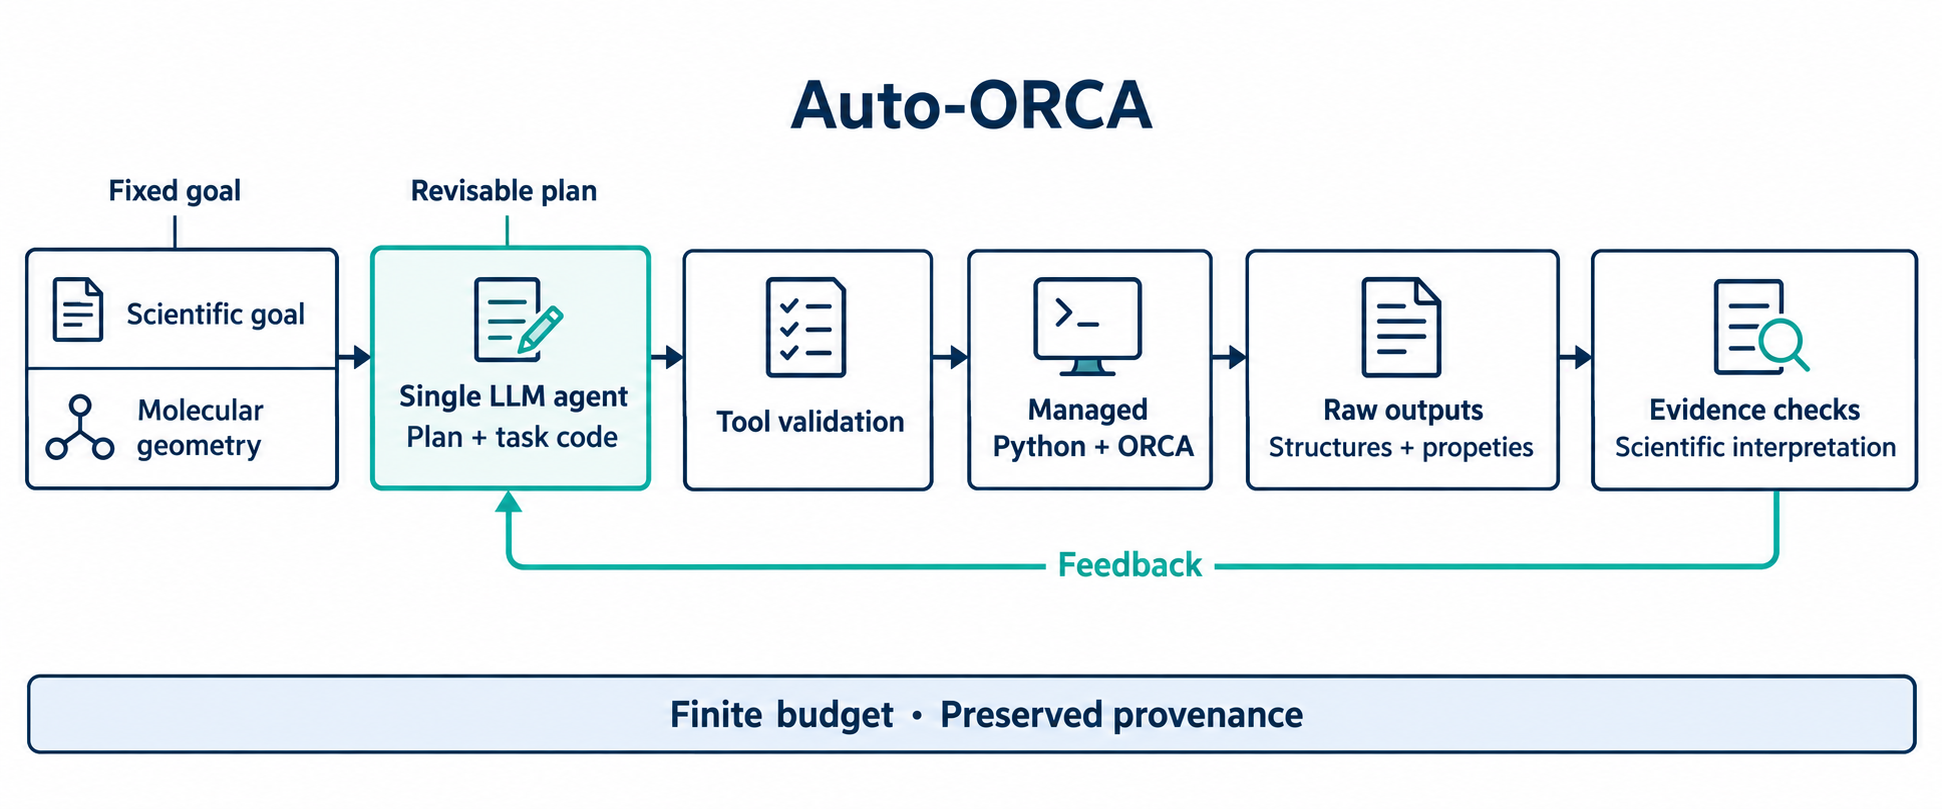
\includegraphics[width=\linewidth]{auto-orca-architecture.png}
  \caption{The single decision loop in Auto-ORCA.
  The original objectives and minimum evidence requirements constrain result evaluation.
  The model uses generic tools to organize managed Python and ORCA execution and revises the plan in response to the returned evidence.}
  \label{fig:architecture}
\end{figure}

Task-specific algorithms are expressed in generated code, while generic tools handle input validation, execution, and artifact management.
For example, a program may construct a finite set of geometries, request an energy calculation for each, and compare the results in consistent units.
OPI input, native ORCA input, and calculation requests issued within Python share the same execution entry point~\cite{opi}.
The thin interface returns execution receipts and raw artifacts without embedding an implicit solution algorithm for an individual problem.
This design allows the same tools to support different tasks while maintaining explicit execution boundaries.

\subsection{Objective Preservation and Evidence Management}
The system uses Request, Plan, Step, Tool, Run, Result, and Artifact to represent requirements, computational routes, operations, execution interfaces, run records, results, and raw artifacts, respectively.
Scientific objectives and minimum evidence requirements are stored independently of the Plan; plan revisions alter only the route used to meet them.

\begin{table}[htbp]
  \centering\small
  \caption{Core representations in Auto-ORCA and their roles in scientific tasks.}
  \label{tab:domain-objects}
  \begin{tabularx}{\linewidth}{>{\raggedright\arraybackslash}p{1.65cm}YY}
    \toprule
    Object & Stored information & Contribution to task reliability\\
    \midrule
    Request & Scientific system, target quantities, conditions, and minimum evidence & Preserves the problem definition and prevents plan revisions from substituting different objectives\\
    Plan & Operation dependencies and the route to the required evidence & Adapts subsequent work to new evidence\\
    Step & Parameters, inputs, and code references for an operation & Defines the scope of the action to be executed\\
    Tool & Interface, execution effects, validation, and output declarations & Converts model intentions into checked operations\\
    Run & Configuration, execution history, and cumulative resource use & Preserves the same cost limits across recovery and retries\\
    Result & Execution facts, checks, observations, and objective evaluation & Distinguishes calculation completion from the scientific meaning of the result\\
    Artifact & Geometries, inputs, programs, and raw outputs & Makes conclusions traceable to specific sources\\
    \bottomrule
  \end{tabularx}
\end{table}

These representations explicitly connect scientific meaning to the execution process.
Explicit user requirements, defaults, inherited conditions, and automatic choices are recorded separately.
Subsequent references to structures or numerical values bind to specific artifacts and their provenance, rather than to a ``latest file'' that may change during execution.
Different objectives for the same molecule may require different environments or electronic states; the software therefore checks conditions for each objective instead of unconditionally merging all settings.

The model proposes actions and repairs, whereas the software determines whether an action is executable and whether its outputs satisfy the prescribed checks.
Initial geometries, inputs, generated programs, and raw outputs from each attempt are stored separately, with provenance bound through content verification.
Reading evidence does not implicitly initiate a calculation or conversion; additional analyses are performed as explicit operations.
Properties not yet covered by standard checks may be retained as observations with provenance, units, and stated limitations, but neither the model nor a task script can independently confer scientific validity on them.

\subsection{Versioned Knowledge Base and On-Demand Retrieval}
\label{sec:knowledge-layer}
Auto-ORCA incorporates domain knowledge queries into the same agent loop, providing traceable references for task planning, input preparation, and result interpretation.
Sources include the official ORCA 6.1 manual~\cite{orcamanual}, OPI 2.0 documentation~\cite{opi}, RDKit 2025.09.6 documentation, and project-maintained guides on input preparation, method selection, and output diagnosis.
Table~\ref{tab:knowledge-sources} summarizes the role of each source category.

\begin{table}[H]
  \centering\small
  \caption{Knowledge sources used by Auto-ORCA and their roles in autonomous calculations.}
  \label{tab:knowledge-sources}
  \begin{tabularx}{\linewidth}{>{\raggedright\arraybackslash}p{2.8cm}YY}
    \toprule
    Source & Main content & Supported decisions\\
    \midrule
    Official ORCA manual & Input structure, methods and basis sets, optimization, frequencies, and properties & Preparing inputs, verifying options, and identifying diagnostic references\\
    OPI and RDKit documentation & Version-specific interfaces and structure-processing procedures & Preparing structures, writing Python task code, and connecting to calculation interfaces\\
    Project task guides & Principles of input preparation, method selection, and output diagnosis & Preserving conditions, organizing execution dependencies, and identifying repair directions\\
    \bottomrule
  \end{tabularx}
\end{table}

The agent answers knowledge queries by retrieving relevant source passages and archiving their documents, versions, source locations, and verification metadata.
Retrieval supports planning, input preparation, diagnosis, and repair as needed.
Specific computational conclusions nevertheless remain grounded in actual ORCA outputs and the corresponding checks.

\subsection{Unified Execution and Observations of Additional Properties}
Although the model can generate task algorithms, execution responsibilities must remain centralized.
Each tool definition specifies parameter constraints, execution effects, and output declarations; OPI, native input, and internal calculation requests follow the same management procedures.
A program may combine several calculations to address a scientific question, but each calculation retains its own input, geometry, execution facts, and artifacts.
Changing the input representation does not alter resource limits or minimum evidence requirements.

Scientific result acquisition also involves distinct levels of evidence.
A readable raw file establishes that evidence is accessible; successful field extraction establishes that a particular datum has been obtained; only the corresponding output checks support interpretation within their defined scope.
For properties not covered by existing checks, generated code may extract and organize observations with provenance, enabling new analytical questions to yield reportable results while retaining their validation status.
This mechanism expands the range of expressible tasks without treating a script's ``pass'' assertion or a normal exit code as a scientific judgment.

For example, tensor-analysis code may read a matrix from raw output and calculate its trace, but reliable interpretation also depends on correct atom indices, coordinate directions, and units.
Similarly, scan code may request calculations at several angles, but a target-angle label alone does not demonstrate that the final geometry satisfies the constraint.
The model proposes an analytical route; actual execution and verifiable evidence jointly delimit the conclusions that the route can support.

\subsection{Feedback, Resources, and Termination}
Feedback preserves the original objectives, current results, and applicable diagnostics, together with queryable evidence sources.
Errors help locate failures in inputs, programs, or numerical solution, while successful outputs help determine whether additional geometry checks, sampling, or cross-result analyses are required.
When the execution state is uncertain, existing facts are reconciled before further action to avoid duplicate launches.

Resource constraints cover generated programs and their internal ORCA calculations.
Let $B_k$ be the limit for budget dimension $k$, $U_k$ the cumulative usage, and $r_k$ the reservation for a new action.
Execution requires
\begin{equation}
  U_k+r_k\leq B_k.
\end{equation}
Internal calculations, code retries, and model-based corrections all contribute to cumulative usage; pausing or resuming does not reset consumption.
Generated code accesses input copies, necessary runtime libraries, and task artifact directories only within a managed task environment.
Completed calculation results and unanswered questions are retained after termination.

Repairs must preserve the original objectives and all evidence that remains valid.
Corrections to input formatting, repairs to code errors, and adjustments to scientific methods have different implications and should be identified separately in subsequent actions.
A failure does not invalidate other completed calculations, and a success does not automatically validate matters that still require examination.
When the origin of an execution is unclear, existing processes and artifacts are reconciled first to avoid unsupported repetition.

These mechanisms allow feedback to affect subsequent actions, while the original scientific conditions, actual evidence, and remaining resources determine the permissible scope of continuation.

\subsection{Comparison of Open-Loop and Closed-Loop Mechanisms}
To clarify the role of result feedback, we distinguish open-loop planning from closed-loop execution~\cite{autodft} and compare the two arrangements in Figure~\ref{fig:open-closed-loop}.
Here, open-loop operation means that the model specifies a complete route at the outset and execution primarily follows predetermined steps and rules.
It may include error detection, rule-based retries, and routine recovery.
Closed-loop operation instead returns newly generated scientific evidence to the model's decision process, allowing the unexecuted portion of the route to change as understanding of the problem develops.

\begin{figure}[htbp]
  \centering
  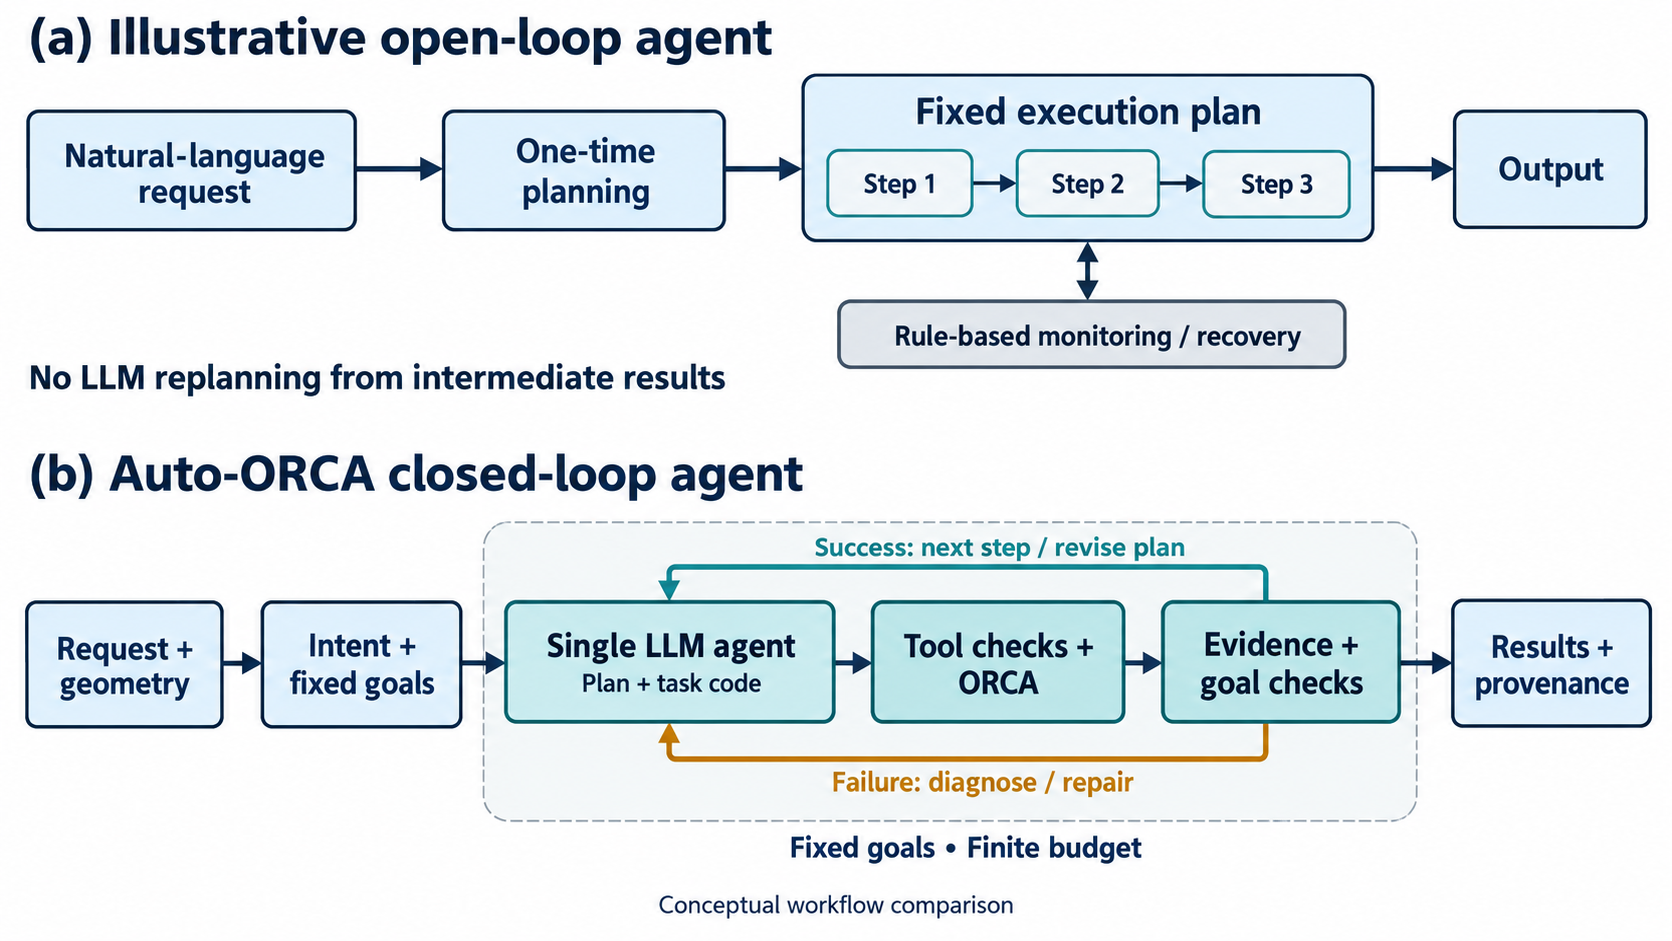
\includegraphics[width=\linewidth]{open-loop-vs-auto-orca.png}
  \caption{Comparison of the mechanisms underlying an open-loop agent and the Auto-ORCA closed-loop workflow.}
  \label{fig:open-closed-loop}
\end{figure}

In molecular calculations, later steps often require information available only after earlier steps have been completed.
For example, frequency analysis must be tied to the optimized structure actually obtained; conformer comparison requires identification of candidates with usable energies; and environmental comparisons require verification that the two calculations share a common geometry.
Returning this information to the decision process after execution allows plans to be grounded in evidence already obtained.
The Auto-ORCA closed loop therefore supports both exception handling and the use of successful results to advance the scientific investigation.

\begin{table}[htbp]
  \centering\small
  \caption{Mechanistic comparison of open-loop operation and Auto-ORCA.}
  \label{tab:loop-comparison}
  \begin{tabularx}{\linewidth}{>{\raggedright\arraybackslash}p{2.35cm}YY}
    \toprule
    Dimension & Illustrative open-loop agent & Auto-ORCA closed-loop organization\\
    \midrule
    Planning & Specifies the complete sequence and main parameters at the outset & Establishes an initial route and determines subsequent actions using new evidence\\
    Successful results & Supply inputs to predetermined steps and predefined post-processing & Also inform objective progress and the suitability of subsequent actions\\
    Exception handling & Monitors, retries, or stops according to predefined rules & Proposes checked repairs using diagnostics, previous attempts, and objectives\\
    Algorithm expression & Executes operations specified in the initial plan & Generates bounded task code for the problem and combines generic tools\\
    Condition preservation & Relies on the initial plan and execution rules & Stores original objectives independently and rechecks conditions after plan revisions\\
    Final delivery & Summarizes outputs from the executed route & Links results, actual conditions, provenance, and unresolved issues to each objective\\
    \bottomrule
  \end{tabularx}
\end{table}

The design advantage of Auto-ORCA lies in the explicit connection between decision-making and execution responsibilities.
A single agent continually addresses the same scientific objectives, generic tools implement each action, and raw artifacts provide a shared basis for subsequent decisions.
Computational, analytical, and interpretive requirements can thus be expressed within a unified task without constructing a separate complete workflow for every combination.
Combining an adaptable route with a stable problem definition provides a basis for gradual extension to more complex potential-energy-surface exploration.

\section{End-to-End Workflow from Natural Language to a Computational Report}
\label{sec:end-to-end-workflow}
Auto-ORCA progressively transforms a user's scientific question into an executable task with explicit inputs, computational conditions, and evidence sources.
The process can be summarized as natural-language input, intent recognition and condition confirmation, objective specification, planning with knowledge retrieval as needed, task code generation, ORCA execution, result checking and feedback, and final delivery.
The same agent loop coordinates these stages.
Because subsequent actions depend on facts already established, the actual route may include evidence queries, plan revisions, and supplementary analyses.
The following subsections describe how information passes between the stages.

\subsection{Natural-Language Input and Scientific Intent Recognition}
The task interface accepts natural-language descriptions together with user-provided structures, output files, or references to existing results.
The system first preserves the original request and identifies four types of information: the system to be studied, the physical quantities required, the conditions that the calculations must satisfy, and the materials the user expects to receive.
For example, ``optimize ethanol and calculate its vibrational frequencies'' must specify the molecular system, structure optimization, frequency calculation at the optimized structure, and delivery of the corresponding coordinates and numerical results.
``Compare the energies of the same structure in two environments'' additionally requires preservation of the common geometry and the pairing between the calculations.

Intent recognition produces a checkable structured candidate that records the system, objectives, geometric relationships, conditions, minimum evidence, and unresolved information.
Key fields retain their supporting source text.
The software checks the correspondence between this candidate and the user message before storing the normalized requirements.
Consequently, qualifiers such as ``the same geometry,'' ``the first five states,'' and ``the complete tensor'' can be preserved throughout the workflow, reducing the risk of recognizing only a broad task category while omitting delivery requirements.

\subsection{Condition Clarification and Objective Specification}
The method, basis set, charge, multiplicity, environment, and geometry source jointly define the actual computational problem.
The system distinguishes conditions explicitly supplied by the user, traceable inherited conditions, defaults, and authorized automatic choices.
Missing information remains recorded as unresolved.
The agent may ask targeted questions when an omission would change the system being calculated or the meaning of the result.
Where the user has delegated method or basis-set selection, the system may record a justified choice and check its compatibility with the remaining conditions before launching the calculation.

Once the conditions have been confirmed, the objectives and minimum evidence requirements are stored independently of the execution plan.
A request may contain multiple objectives, each with its own constraints on the system, environment, electronic state, and geometric relationships.
For example, a comparison of gas-phase and solution energies must preserve two environment-specific objectives and their common geometry; it cannot be reduced to an undifferentiated ``energy'' field.
Fixing the objectives preserves flexibility in the computational route: the plan may add parsing steps or repair inputs, but it must still address the original scientific question.

\subsection{On-Demand Knowledge Queries to Support Operations}
\label{sec:knowledge-retrieval}
When the next operation requires additional information on software syntax, methods, or property definitions, the agent formulates a specific query from the current uncertainty.
The query process comprises source selection, search-term formulation, retrieval of matching passages, and assessment of whether those passages support the current decision.
For example, preparing a frequency task may require consulting documentation on optimization and vibrational analysis; writing Python task code may require the interface documentation for the relevant OPI version; and diagnosing an input error may use the ORCA log to locate the relevant manual section.

Knowledge queries may also be used after results have been returned.
For example, references can help establish the meaning of physical quantities when explaining the relationship between nuclear magnetic shielding and chemical shifts or distinguishing electronic energy differences from free energies.
The numerical values, geometries, and convergence states of existing results are instead read from their corresponding raw artifacts.
The final report can therefore state the basis for an operation, the actual computational conditions, and the sources of its numerical results.

\subsection{Organizing the Computational Plan by Dependencies}
The agent next translates the objectives into interdependent operations, including reading or preparing structures, generating inputs, executing calculations, extracting properties, and organizing results.
Each step identifies the system to be used, the registered files it consumes, the tool it invokes, and the outputs it is expected to provide.
The software checks the relationship between the plan and the objectives, file dependencies, tool permissions, and available budgets.
An operation becomes eligible for execution only when its prerequisite data are available and satisfy the checks required by that step.

The plan translates scientific ordering requirements into data dependencies.
A frequency calculation after optimization must obtain the corresponding final structure; candidate energy ranking must preserve the association between each energy and its candidate identifier; and rotational consistency analysis requires results for two orientations together with the rotation definition.
When the route must change, the system creates a new plan version while preserving the original records of executed inputs and attempts.
This allows exploration to adapt to new information while retaining an explanation of the route that produced each result.

\subsection{Task Code Generation through a Unified Tool Boundary}
For tasks that are difficult to express directly through fixed interfaces, the agent may write Python task code and native ORCA input to perform repeated calculations, extract fields, organize matrices, or analyze deterministic derived quantities.
Code is first stored as a file with provenance and then referenced by an execution step.
Before execution, the system checks the identities of the code and inputs, file dependencies, and task declarations.
Generated programs run in a managed environment, and internal ORCA requests continue to pass through the unified entry point.

With this organization, new tasks are expressed primarily through changes in operation composition and task programs.
For example, conformer comparison requires managing a set of geometries and energies; excited-state analysis requires organizing state-resolved outputs; and shielding analysis requires preserving atom indices and matrix components.
All three can use the same mechanisms for file writing, execution, querying, and archiving.
Programs provide general computational capabilities, while the tool boundary maintains traceability of actual inputs, resource consumption, and raw artifacts.

\subsection{Execution, Monitoring, and Raw Artifact Archiving}
Before launch, the system verifies the actual inputs, geometry, conditions, permissions, and remaining resources, and creates a separate record for the operation.
Task code and its internal ORCA calculations share a controlled execution environment and cumulative resource constraints.
Launch is confirmed by a trusted execution receipt.
If the execution state is uncertain, existing processes and receipts are reconciled first, preventing an unknown state from being mistaken for a calculation that has not started and thereby duplicated.

After execution, the system archives inputs, standard output, error logs, structure files, and property files, and links each result to its raw artifacts.
Records are preserved for both normal completion and failure.
They provide specific objects for subsequent diagnosis and allow successful numerical results and failure causes to enter the same feedback process.

\subsection{Result Checking and Evidence-Based Continuation}
After receiving a new result, the main loop reevaluates the objectives before deciding on the next action.
Checks cover the actual conditions, file integrity, output readability, and applicable scientific validation.
Outputs covered by existing checks are evaluated according to their corresponding rules; new properties may be extracted by task code as observations with provenance, units, and validation statements.
Successful result reading, calculation completion, reportable observations, and verified scientific requirements are recorded separately so that final conclusions correspond to the evidence actually obtained.

Successful feedback may initiate a further necessary analysis.
For example, completed optimization must be followed by acquisition of the final structure and frequency evidence, while completed candidate calculations require consolidation of their associations and consistent energy units.
Failure feedback includes specific fields, program errors, or locations in ORCA logs so that the agent can propose targeted repairs.
When software documentation must be checked, the feedback can support a focused knowledge query whose findings inform the proposed revision.
Repairs use new inputs or subsequent steps while preserving the original objectives and sources that remain valid; the original failure remains accessible.

The system also checks whether executable work remains for the current objectives.
When approved subsequent steps, recoverable failures, or analytical routes based on archived originals remain available, feedback identifies the corresponding continuation options, and the final delivery check uses this information to prevent premature termination.
If existing files already support the required analysis, continuation may require only an additional parsing operation.
This mechanism connects calculation with analysis and directs further effort toward identified evidence gaps.

\subsection{Final Output and Verifiable Delivery}
When the task reaches a deliverable state, or when resources, permissions, or specific execution conditions require termination, the system consolidates the correspondence between objectives and evidence.
The final output includes the question and actual methods, the numerical results or structures obtained, necessary units and reference definitions, calculation and validation status, artifact locations, and outstanding work.
Method-selection rationales refer directly to saved records, while numerical values are traced to the corresponding raw outputs and analytical sources.
Knowledge sources used during the task are linked through retrieval records to document versions and passage locations, preserving traceability of both the operational rationale and the result sources.

For the user, this delivery provides a continuous path from posing a question to obtaining computational materials suitable for further use.
Tables facilitate comparison, raw files support verification, and limitations indicate what additional evidence is needed.
The calculation success rate used in this report describes whether corresponding ORCA calculations for the seven questions completed normally and produced numerical results.
The scientific conclusions supported by each result remain separately delimited by its method, geometry, and property evidence.

\subsection{Illustration: Information Flow in Ethanol Optimization and Frequency Analysis}
Using ethanol optimization and vibrational frequency analysis as an illustrative example, the table below traces the information flow from a natural-language request to final delivery.

\begin{table}[htbp]
  \centering\small
  \caption{Progressive specification of information in the ethanol task.
  The illustrative natural-language input is ``Optimize neutral singlet ethanol in the gas phase using r$^{2}$SCAN-3c and report its vibrational frequencies.''}
  \label{tab:workflow-example}
  \begin{tabularx}{\linewidth}{>{\raggedright\arraybackslash}p{2.35cm}YY}
    \toprule
    Stage & Information established & Information passed to the next stage\\
    \midrule
    Intent recognition & Ethanol; structure optimization; vibrational frequencies & Two types of results and the requirement to calculate frequencies at the optimized structure\\
    Condition confirmation & Gas phase, neutral singlet, r$^{2}$SCAN-3c & Confirmed method, built-in basis set, and geometry source\\
    On-demand knowledge queries & Relevant references on the method, interface, or frequency settings & Citable source passages, software versions, and operational rationale\\
    Planning & Structure preparation, calculation, extraction, and interpretation & Inputs and required outputs for each operation\\
    Code and input & Actual ORCA input and any required analysis programs & File identities, conditions, and resource declarations\\
    Execution and archiving & Raw outputs, final coordinates, and property files & Actual completion status and readable artifacts\\
    Checking and analysis & Convergence records, mode count, and imaginary frequencies & Evidence concerning energy, frequencies, and local stability\\
    Result delivery & Methods, numerical values, coordinates, and interpretation & Readable conclusions and computational materials available for further use\\
    \bottomrule
  \end{tabularx}
\end{table}

% !TeX root = main.tex
\section{Computational Methods and Agent Capability Assessment}
\subsection{Computational Settings and Scientific Tasks}
Calculations were performed using ORCA 6.1.1 and organized through OPI 2.0.0 and the unified execution interface.
The local resource allocation comprised four CPU cores, a memory limit of 1024 MiB for the computational process tree,
and an ORCA MaxCore setting of 192 MiB per process.
MaxCore is an internal ORCA memory parameter and was configured separately from the total memory limit on the process tree.

Table~\ref{tab:task-overview} lists the methods actually used for the seven test problems.
All systems for which calculations were completed were neutral singlets.
The r$^{2}$SCAN-3c calculations used the built-in def2-mTZVPP basis set~\cite{r2scan3c};
other methods and basis sets are reported individually according to the calculations performed,
with the basis sets following the def2 definitions~\cite{def2}.
Vertical excitations were calculated using full linear-response TDDFT~\cite{tddft},
and the aqueous environment was represented by the CPCM continuum model~\cite{cpcm}.
Except for the explicitly identified geometry optimizations and constrained optimizations,
all results correspond to specified fixed geometries.

\subsection{Design of the Agent Capability Assessment}
\label{sec:agent-evaluation-design}
The seven problems below assess \textbf{the ability of the Auto-ORCA agent to translate scientific requests
into actual calculations and interpretable results}.
The assessment covers the full process, from task interpretation, preservation of conditions,
and input preparation to the organization of results.
The molecules and properties were selected to impose distinct operational requirements:
some problems require a structure to be obtained before a property can be calculated;
others require management of a finite candidate set, preservation of comparable conditions,
organization of multiple excited states, or tensor analysis.
Together, these problems constitute a set of capability checks that examine both whether the agent can initiate and complete
actual ORCA calculations and whether its deliverables clearly identify the calculated system, conditions, and scope of the conclusions.

The test set includes operations relevant to potential energy surfaces as well as property calculations.
T1--T3 address local structure determination, comparison of candidate geometries,
and constrained calculations along an internal coordinate, respectively.
These are common components of potential energy surface exploration.
T4, T5, H1, and H2 extend the assessment to excited states, environmental changes, and response tensors,
testing whether the same execution interface can support different forms of output.
Task identifiers serve only to associate problems with their results;
capability assessments are based on the actual inputs, outputs, and geometry records.
Table~\ref{tab:agent-capability-design} specifies the capabilities targeted by each problem and the evidence that requires examination.

\begin{figure}[htbp]
  \centering
  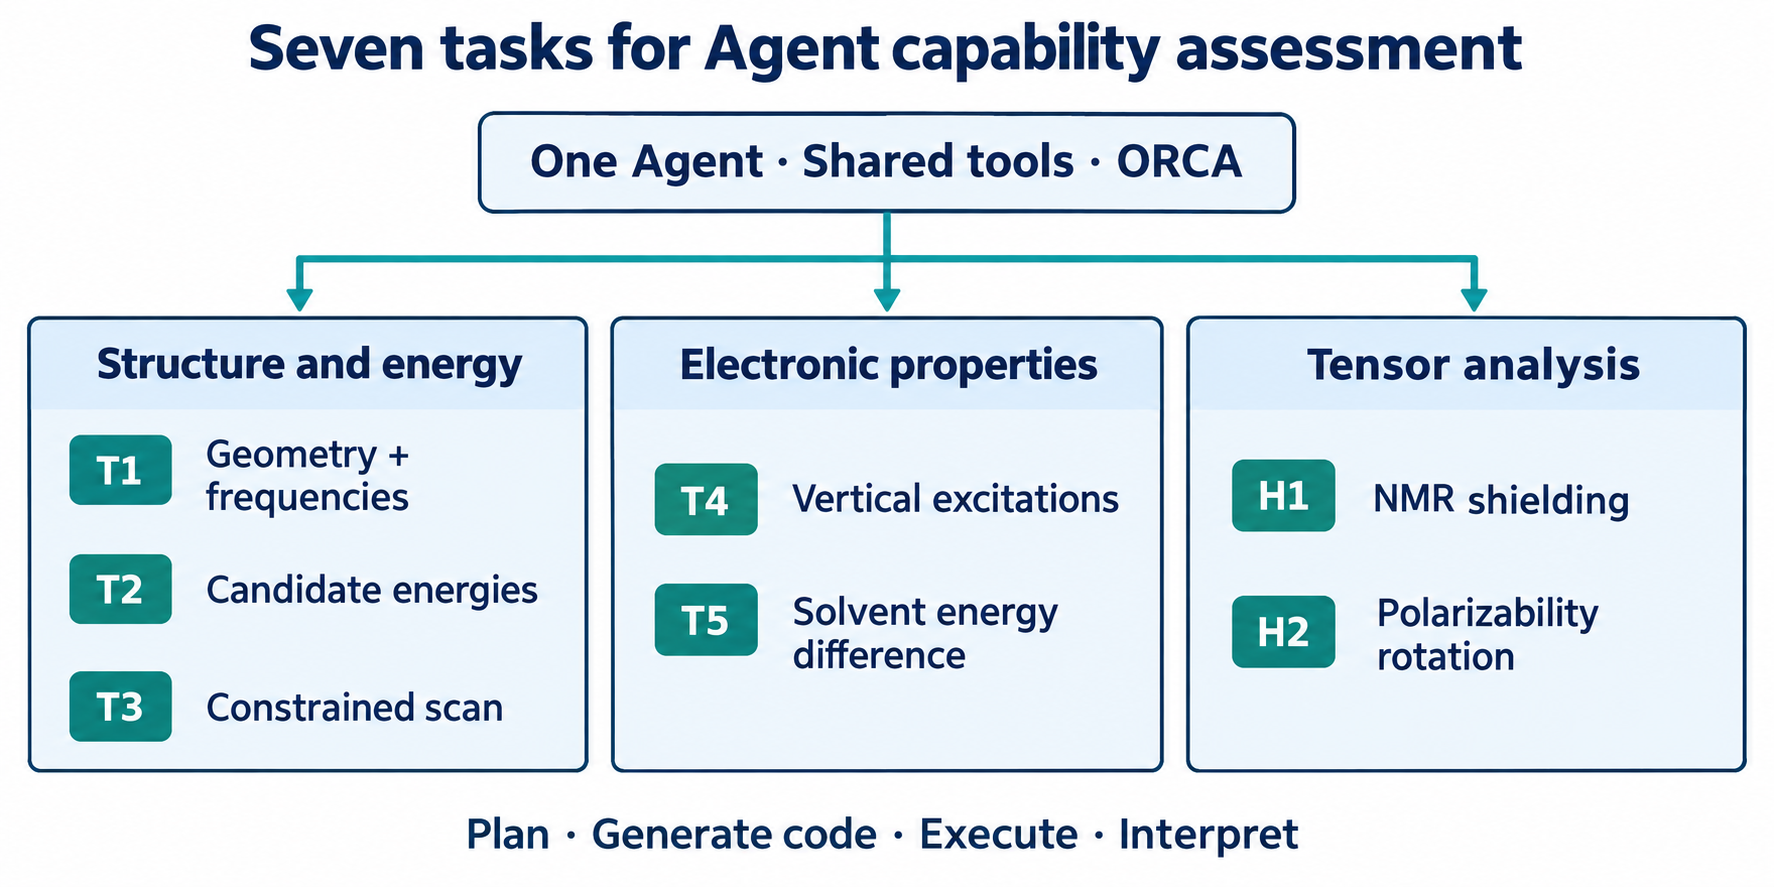
\includegraphics[width=\linewidth]{agent-capability-map.png}
  \caption{Scope of the agent capability assessment across seven problems.
  All problems use the same task organization and ORCA execution mechanism,
  while examining distinct operational requirements for structures and energies, electronic properties, and tensor analysis.
  The diagram illustrates the assessment design; the extent of completion is determined by the actual results.}
  \label{fig:agent-capability-map}
\end{figure}

\begin{table}[htbp]
  \centering\small
  \caption{Design of the agent capability assessment.
  The table lists the intended assessment dimensions; the extent of completion is reported with the individual results.}
  \label{tab:agent-capability-design}
  \begin{tabularx}{\linewidth}{lYY}
    \toprule
    Task & Principal capability & Evidence to examine\\
    \midrule
    T1 & Organize optimization--frequency dependencies and preserve structural provenance
       & Optimization convergence, final geometry, frequency count, and imaginary frequencies\\
    T2 & Organize a finite set of candidate calculations, associate identifiers, and standardize energy units
       & Candidate geometries, individual energies, reference candidate, and unit conversions\\
    T3 & Generate a loop for constrained calculations and maintain correspondence between target inputs and actual geometries
       & Constraint inputs, outputs at each point, final dihedral angles, and incomplete points\\
    T4 & Configure native property calculations and associate outputs across excited states
       & Method and TDA settings, convergence records, state-resolved energies, and oscillator strengths\\
    T5 & Preserve comparable geometries and methods when changing the environment
       & Geometries in both environments, basis and solvent settings, and the sign of the energy difference\\
    H1 & Parse atom-resolved tensors while preserving units and component ordering
       & Atom indices, complete shielding matrices, isotropic values, and units of ppm\\
    H2 & Organize calculations before and after rotation and check tensor consistency
       & Both molecular orientations, rotation definition, polarizability tensors, and comparison residuals\\
    \bottomrule
  \end{tabularx}
\end{table}

\FloatBarrier

Results can be examined at three levels.
First, the actual method, geometry, charge, and multiplicity are checked to associate each result with a well-defined computational problem.
Second, the raw ORCA output is examined for normal termination and the requested numerical values are checked for actual preservation.
Third, the interpretation is assessed against the available evidence.
For example, the lowest single-point energy in a finite candidate set must not be described as the global minimum conformer,
and an electronic energy difference at a fixed geometry must not be described as a free energy.
The first two levels establish the provenance of the computational system and its outputs;
the third determines the extent to which those outputs answer the scientific question.

Accordingly, Table~\ref{tab:agent-capability-design} specifies the dimensions covered by the assessment,
rather than a set of capabilities that have all been demonstrated successfully.
The completed calculations provide examples of diverse task formulations, execution, and numerical delivery.
A more complete assessment still requires individual verification of dependencies, geometric correspondence, and property interpretation.
The seven-problem success rate also lacks the statistical evidence provided by repeated trials or comparison systems
and therefore cannot estimate the probability of success on unseen tasks.
Future evaluations can repeat these problems under identical goals and conditions,
resolve the remaining verification gaps, and distinguish computational completion, verifiability of results,
and fulfillment of the scientific goals.

\subsection{Calculation Success Rate and Interpretation of Results}
Normal-termination records in the raw ORCA output serve as evidence that a calculation has completed.
Each problem in this study is classified as \textbf{successful} if a corresponding ORCA calculation has terminated normally
and its numerical results have been retained; a problem with no actual numerical result is classified as \textbf{incomplete}.
This classification includes the six completed points in T3 despite the uncomputed endpoint and the limitations of angle verification.
\begin{equation}
  R_{\mathrm{calc}}=\frac{N_{\mathrm{success}}}{N_{\mathrm{questions}}}
  =\frac{6}{7}\approx85.7\%.
  \label{eq:success-rate}
\end{equation}
The denominator is the set of seven problems, with each problem counted once.
Scientific conclusions are interpreted separately using the available evidence on convergence, geometry, method, and property.
Normal termination alone does not establish a global minimum conformer, a correct torsional barrier,
or a response property that can be compared directly with experiment.

Relative electronic energies are referenced to a specified member of the candidate set.
Energy conversions use $1\,\Eh=2625.4996394799$ kJ mol$^{-1}$.
Electronic energies, vibrational frequencies, excitation energies, and shielding tensors retain the precision
of the original output or verification record.
Raw data and provenance records support inspection and reuse~\cite{fair}.
This report presents existing computational results; the reported success rate is not interpreted as a success probability
for arbitrary new tasks, and energy differences without independent references are not used to assess methodological accuracy.

\subsection{Scope of the Evaluation}
The calculation success rate across the seven problems indicates whether the agent has produced actual computational results for those problems.
Assessing numerical accuracy additionally requires confirmation that each calculated value and its independent reference
refer to the same system, geometry, physical quantity, and theoretical conditions.
For tasks with reliable reference values, the coverage of valid matches and the error over the matched subset can be reported separately:
\begin{equation}
  \mathrm{Coverage}=\frac{N_{\mathrm{matched}}}{N_{\mathrm{target}}},
  \qquad
  \mathrm{MAE}_{\mathrm{matched}}=
  \frac{1}{N_{\mathrm{matched}}}\sum_{i\in\mathcal M}|y_i-y_i^{\mathrm{ref}}|.
  \label{eq:coverage-accuracy}
\end{equation}
Here, $\mathcal M$ includes only targets whose correspondence has been established,
and $y_i$ and $y_i^{\mathrm{ref}}$ are expressed in the same units.
If $N_{\mathrm{matched}}=0$, the error is not evaluable.
This formulation specifies the conditions required for future accuracy comparisons.
No independent high-accuracy references are available in this study; consequently, no empirical MAE is reported,
and energy differences between distinct methods or geometries are not treated as numerical errors.

\section{Results of the Agent Capability Assessment}
% !TeX root = main.tex
\subsection{Overview of the Seven Test Cases}
The following seven scientific questions were used to evaluate the task organization and execution capabilities of Auto-ORCA Agent;
their intended capability coverage is summarized in Table~\ref{tab:agent-capability-design}.
Table~\ref{tab:task-overview} summarizes the methods actually used and the results obtained for each case.
T1--T5 and H1 were classified as successful calculations, whereas H2 remained incomplete, yielding a calculation success rate of $6/7=85.7\%$.
The numerical results and their scientific interpretation are presented below.

\begin{table}[H]
  \centering\small
  \caption{Methods actually used and results obtained for the seven test cases.
  Success indicates that an ORCA calculation terminated normally and produced the corresponding numerical results.
  }
  \label{tab:task-overview}
  \begin{tabularx}{\linewidth}{l>{\raggedright\arraybackslash}p{2.6cm}>{\raggedright\arraybackslash}p{3.1cm}>{\raggedright\arraybackslash}p{1.8cm}Y}
    \toprule
    ID & Question & Actual method & Status & Principal results\\
    \midrule
    T1 & Ethanol optimization and frequencies & r$^{2}$SCAN-3c & Success & Converged optimization; 21 positive frequencies and no imaginary frequencies\\
    T2 & Candidate energies for \textit{n}-hexane & r$^{2}$SCAN-3c single-point calculations & Success & Energy ranking of six candidate geometries\\
    T3 & Dihedral scan of \textit{n}-butane & r$^{2}$SCAN-3c constrained optimization & Success & Six converged points; actual angles remain unverified\\
    T4 & Vertical excitations of acetone & PBE0/def2-SVP, LR-TDDFT & Success & Five singlet excitation energies and oscillator strengths\\
    T5 & Environmental energy differences for ethanol & B3LYP/def2-TZVP and def2-SVP & Success & Gas-phase--CPCM water electronic energy differences with two basis sets\\
    H1 & Nuclear magnetic shielding of HCN & PBE0/def2-TZVP, GIAO & Success & Full shielding tensors for the C, N, and H nuclei\\
    H2 & Formaldehyde polarizability and rotational consistency & No actual calculation results & Incomplete & No polarizability values obtained\\
    \bottomrule
  \end{tabularx}
\end{table}

\subsection{T1: Geometry Optimization and Vibrational Frequencies of Ethanol}
\paragraph{Question}
Optimize the geometry of ethanol and use its vibrational frequencies to assess whether the resulting structure is a local minimum.

\paragraph{Method}
Geometry optimization and vibrational frequency calculations were performed using r$^{2}$SCAN-3c with its built-in def2-mTZVPP basis set for a neutral singlet in the gas phase.

\paragraph{Results}
\textbf{Successful calculation.} The geometry optimization converged, giving an optimized electronic energy of $-155.002345492244\,\Eh$.
The calculation yielded 21 positive vibrational frequencies, six zero-frequency translational and rotational modes after projection, and no imaginary frequencies.
All positive frequencies are listed in Table~\ref{tab:t1-frequencies}.
These results support assignment of the structure as a local minimum at the employed level of theory; they do not establish that it is the global minimum-energy conformer.
The optimized coordinates are retained in the XYZ file associated with the corresponding ORCA output.

\begin{table}[H]
  \centering\small
  \caption{The 21 positive vibrational frequencies of ethanol, in cm$^{-1}$.}
  \label{tab:t1-frequencies}
  \begin{tabular}{rrrrrrr}
    \toprule
    270.90 & 298.95 & 425.86 & 811.51 & 882.13 & 1052.13 & 1066.45\\
    1134.41 & 1282.25 & 1371.13 & 1396.18 & 1418.25 & 1483.33 & 1487.57\\
    1509.53 & 2969.59 & 3004.65 & 3061.83 & 3088.36 & 3105.66 & 3819.31\\
    \bottomrule
  \end{tabular}
\end{table}

\subsection{T2: Single-Point Electronic Energies of Candidate \textit{n}-Hexane Conformers}
\paragraph{Question}
Compare the electronic energies of candidate \textit{n}-hexane geometries and determine their relative energy ordering within the calculated set.

\paragraph{Method}
Single-point calculations were performed separately for six stored candidate geometries using r$^{2}$SCAN-3c for neutral singlets in the gas phase.
Relative energies were referenced to cand\_05.

\paragraph{Results}
\textbf{Successful calculation.} Electronic energies were obtained for all six candidates, as reported in Table~\ref{tab:t2-energies}.
Within this set, cand\_05 had the lowest energy, whereas cand\_03 was higher by 12.608656~kJ~mol$^{-1}$.
These are single-point results for candidate geometries; they do not demonstrate that all six conformers underwent DFT optimization,
nor do they establish the global minimum-energy conformer or a free-energy ordering.

\begin{table}[H]
  \centering\small
  \caption{Single-point electronic energies of six candidate \textit{n}-hexane geometries.}
  \label{tab:t2-energies}
  \begin{tabular}{lrr}
    \toprule
    Candidate & Electronic energy / $\Eh$ & Relative energy / kJ mol$^{-1}$\\
    \midrule
    cand\_05 & $-236.992066202851$ & 0.000000\\
    cand\_04 & $-236.991445556657$ & 1.629506\\
    cand\_01 & $-236.991444090308$ & 1.633356\\
    cand\_00 & $-236.991421448668$ & 1.692802\\
    cand\_06 & $-236.991245997872$ & 2.153448\\
    cand\_03 & $-236.987263819406$ & 12.608656\\
    \bottomrule
  \end{tabular}
\end{table}

\subsection{T3: Dihedral Scan of \textit{n}-Butane}
\paragraph{Question}
Obtain the electronic energies of \textit{n}-butane at different target dihedral angles through constrained optimization and examine the variation in torsional potential energy.

\paragraph{Method}
The main calculations employed r$^{2}$SCAN-3c for a neutral singlet in the gas phase, with constrained optimization at specified target dihedral angles.
An additional B3LYP/def2-TZVP calculation point is reported separately, together with the result of its geometry verification.

\paragraph{Results}
\textbf{Successful calculation.} Normal ORCA termination and optimization convergence were recorded for all six r$^{2}$SCAN-3c calculation points;
the results are given in Table~\ref{tab:t3-energies}.
The first column contains only the target-angle labels specified in the inputs.
The actual angles reported by the generated script conflict with these input labels and have not yet been confirmed through independent geometry verification.
Consequently, the energies are genuine computational outputs, but the labels cannot be treated as verified actual dihedral angles or used to establish a torsional barrier.
In particular, the high energy associated with the $+120^\circ$ label cannot be directly interpreted as a reliable physical barrier.

\begin{table}[H]
  \centering\small
  \caption{Six constrained optimization points for \textit{n}-butane.
  Angles denote input target labels; relative energies are the stored numerical values.
  }
  \label{tab:t3-energies}
  \begin{tabular}{rrr}
    \toprule
    Input target angle / $^\circ$ & Electronic energy / $\Eh$ & Relative energy / kJ mol$^{-1}$\\
    \midrule
    $-180$ & $-158.392470368263$ & 0.000000\\
    $-120$ & $-158.387146187943$ & 13.978634\\
    $-60$ & $-158.391526560891$ & 2.477966\\
    $0$ & $-158.383528626170$ & 23.476541\\
    $+60$ & $-158.391526702130$ & 2.477595\\
    $+120$ & $-158.358972460497$ & 87.948745\\
    \bottomrule
  \end{tabular}
\end{table}

The input target angle for the B3LYP/def2-TZVP calculation point was $-180^\circ$.
Independent geometry verification gave an actual angle of $179.999995786^\circ$, consistent with the target under angular periodicity;
the converged electronic energy was $-158.397118300397\,\Eh$.
Because this point was obtained using a different method, it is excluded from the relative energies in Table~\ref{tab:t3-energies}.

\subsection{T4: The First Five Singlet Vertical Excitations of Acetone}
\paragraph{Question}
Obtain the excitation energies, wavelengths, and oscillator strengths of the first five singlet vertical excitations of acetone.

\paragraph{Method}
Five singlet excited states were calculated at a fixed, prepared geometry using PBE0/def2-SVP for a neutral singlet in the gas phase,
with full linear-response TDDFT (LR-TDDFT; \code{TDA=false}).
Oscillator strengths were taken from the length-gauge output of ORCA.

\paragraph{Results}
\textbf{Successful calculation.} Convergence was recorded for both the SCF and response calculations; numerical results for the five excited states are listed in Table~\ref{tab:t4-excitations}.
The lowest singlet vertical excitation energy was 4.197061~eV, corresponding to a wavelength of 295.4~nm.

\begin{table}[H]
  \centering\small
  \caption{The first five singlet vertical excitations of acetone.
  Oscillator strengths $f$ are dimensionless.
  }
  \label{tab:t4-excitations}
  \begin{tabular}{crrr}
    \toprule
    Excited state & Excitation energy / eV & Wavelength / nm & Oscillator strength $f$\\
    \midrule
    $S_{1}$ & 4.197061 & 295.4 & 0.000007493\\
    $S_{2}$ & 7.464499 & 166.1 & 0.023781213\\
    $S_{3}$ & 8.406988 & 147.5 & 0.001899769\\
    $S_{4}$ & 8.572306 & 144.6 & 0.060276158\\
    $S_{5}$ & 8.640904 & 143.5 & 0.004121254\\
    \bottomrule
  \end{tabular}
\end{table}

\subsection{T5: Electronic Energy Differences between Gas-Phase Ethanol and Ethanol in CPCM Water}
\paragraph{Question}
Compare the electronic energies of ethanol at the same geometry in the gas phase and in a CPCM water environment.

\paragraph{Method}
Calculations employed B3LYP for a neutral singlet with the def2-TZVP and def2-SVP basis sets, respectively.
For each basis set, the gas-phase and aqueous-environment calculations used the same initial geometry; this geometry was not the optimized structure from T1.
The energy difference was defined as $\Delta E=E_{\mathrm{water}}-E_{\mathrm{gas}}$.

\paragraph{Results}
\textbf{Successful calculation.} Two ORCA calculations, one in the gas phase and one in CPCM water, were completed for each basis set.
Table~\ref{tab:t5-energies} reports the electronic energies, and Table~\ref{tab:t5-differences} reports their differences.
The negative signs indicate that, for the corresponding model and fixed geometry, the electronic energy in the aqueous environment was lower than that in the gas phase.
These quantities are \textbf{electronic energy differences, not hydration free energies}.

\begin{table}[H]
  \centering\small
  \caption{Electronic energies of ethanol in the gas phase and in CPCM water.}
  \label{tab:t5-energies}
  \begin{tabular}{lrr}
    \toprule
    Basis set & Gas-phase electronic energy / $\Eh$ & CPCM water electronic energy / $\Eh$\\
    \midrule
    def2-TZVP & $-155.002778990957$ & $-155.009740144896$\\
    def2-SVP & $-154.817054999208$ & $-154.823380641772$\\
    \bottomrule
  \end{tabular}
\end{table}

\begin{table}[H]
  \centering\small
  \caption{Electronic energy differences for ethanol in water relative to the gas phase.}
  \label{tab:t5-differences}
  \begin{tabular}{lrr}
    \toprule
    Basis set & $\Delta E$ / $\Eh$ & $\Delta E$ / kJ mol$^{-1}$\\
    \midrule
    def2-TZVP & $-0.006961153939$ & $-18.276507$\\
    def2-SVP & $-0.006325642564$ & $-16.607972$\\
    \bottomrule
  \end{tabular}
\end{table}

\subsection{H1: GIAO Nuclear Magnetic Shielding Tensors of HCN}
\paragraph{Question}
Obtain the nuclear magnetic shielding tensor and isotropic shielding of each atom in HCN.

\paragraph{Method}
Calculations were performed at a fixed initial geometry using PBE0/def2-TZVP and the GIAO method for a neutral singlet in the gas phase.
The atom order was C$_0$, N$_1$, and H$_2$.

\paragraph{Results}
\textbf{Successful calculation.} The total electronic energy was $-93.345070922944\,\Eh$.
The isotropic shielding values printed by ORCA are listed in Table~\ref{tab:h1-isotropic}; the full total shielding tensors are given in Eq.~\eqref{eq:h1-tensors}.
The tensor components are expressed in ppm, with both rows and columns ordered as X, Y, and Z; the three decimal places of the original output are retained.

\begin{table}[H]
  \centering\small
  \caption{Isotropic nuclear magnetic shielding values for HCN.}
  \label{tab:h1-isotropic}
  \begin{tabular}{cr}
    \toprule
    Atom & Isotropic shielding / ppm\\
    \midrule
    C$_0$ & 79.051\\
    N$_1$ & $-34.068$\\
    H$_2$ & 29.850\\
    \bottomrule
  \end{tabular}
\end{table}

\begin{equation}
  \begin{aligned}
    \bm{\sigma}_{\mathrm{C}_0}&=\begin{pmatrix}
      279.306 & -0.724 & -0.000 \\
      -1.638 & -21.077 & 0.000 \\
      -0.000 & 0.000 & -21.076
    \end{pmatrix},\\[0.8em]
    \bm{\sigma}_{\mathrm{N}_1}&=\begin{pmatrix}
      340.398 & -1.842 & -0.000 \\
      -0.044 & -221.291 & 0.000 \\
      0.000 & 0.000 & -221.309
    \end{pmatrix},\\[0.8em]
    \bm{\sigma}_{\mathrm{H}_2}&=\begin{pmatrix}
      39.712 & 0.055 & -0.000 \\
      -0.114 & 24.919 & -0.000 \\
      -0.000 & -0.000 & 24.920
    \end{pmatrix}.
  \end{aligned}
  \label{eq:h1-tensors}
\end{equation}
Isotropic shielding is one-third of the tensor trace; the tabulated values were taken directly from the summary printed by ORCA and were not recalculated from the rounded matrices.
These quantities have not been converted using a reference compound and therefore cannot be directly described as experimental chemical shifts.
H$_2$ denotes the index of the hydrogen atom and is unrelated to the task identifier H2 in the following subsection.

\subsection{H2: Static Polarizability and Rotational Consistency of Formaldehyde}
\paragraph{Question}
Obtain the static polarizability tensors and isotropic polarizabilities of formaldehyde in two orientations, and assess their physical consistency under rotation.

\paragraph{Method}
The geometries and rotation procedure were prepared, with the intention of calculating the polarizability in each orientation and comparing the results after coordinate transformation.

\paragraph{Results}
\textbf{Incomplete.} No actual ORCA polarizability values have been obtained.
Consequently, neither the polarizability tensors and isotropic polarizabilities in the two orientations nor a rotational consistency comparison is available.
The prepared geometries and rotation procedure do not constitute calculation results.

\paragraph{Analysis of the Failure}
The execution records indicate that interruption occurred primarily during task orchestration and data handoff before the calculation.
In the recorded attempts, an identity-description file was incorrectly bound as an XYZ geometry input, causing the rotation preprocessing script to terminate abnormally during coordinate parsing.
The identification and use of diagnostic information did not yield an effective repair; the corresponding runs terminated upon reaching either the model-call limit or the finite allowance for plan revisions.


\subsection{Agent Token Usage and Costs for Runs Producing Computational Results}
\label{sec:token-cost}
To characterize the model resources required for autonomous task organization,
Table~\ref{tab:token-cost} lists six runs that produced the ORCA numerical results reported above.
Input, output, and total token counts were accumulated from the provider's per-call usage records
and cross-checked against the usage records for the corresponding runs.
The counts cover each entire agent run, including task interpretation, input preparation, planning decisions,
code repair, analysis, and reporting.
ORCA itself consumes computational resources rather than language-model tokens.
Because model calls and ORCA jobs do not correspond one-to-one, their counts are listed separately.

\begin{table}[H]
  \centering\small
  \setlength{\tabcolsep}{4pt}
  \caption{Agent token usage and estimated off-peak costs for runs that produced ORCA results.
  Token usage records are complete for all six runs.
  Costs are estimated uniformly using DeepSeek Flash rates and the recorded cache usage, and are expressed in USD.}
  \label{tab:token-cost}
  \begin{tabular*}{\linewidth}{@{\extracolsep{\fill}}lrrrrrr@{}}
    \toprule
    Task & \shortstack[r]{ORCA\\jobs} & \shortstack[r]{Model\\calls} & \shortstack[r]{Input\\tokens} & \shortstack[r]{Output\\tokens} & \shortstack[r]{Total\\tokens} & \shortstack[r]{Off-peak\\estimate}\\
    \midrule
    T1 & 1 & 21 & 311,695 & 86,697 & 398,392 & 0.079900\\
    T2 & 6 & 12 & 181,958 & 49,010 & 230,968 & 0.049813\\
    T3 & 6 & 14 & 231,346 & 107,149 & 338,495 & 0.092519\\
    T4 & 1 & 23 & 367,183 & 75,633 & 442,816 & 0.087719\\
    T5 & 2 & 12 & 192,013 & 62,392 & 254,405 & 0.063885\\
    H1 & 1 & 24 & 368,095 & 117,100 & 485,195 & 0.114298\\
    \bottomrule
  \end{tabular*}
\end{table}

All six cost estimates use the rates for \code{deepseek-flash}.
The rates for cached input, uncached input, and output are 0.003, 0.15, and 0.60 USD per million tokens, respectively.
Let $N_{\mathrm{hit}}$ denote the cached input tokens already included in the total input count.
The cost is then estimated as
\begin{equation}
  C_{\mathrm{off\text{-}peak}}=
  \frac{p_{\mathrm{hit}}N_{\mathrm{hit}}
  +p_{\mathrm{miss}}(N_{\mathrm{input}}-N_{\mathrm{hit}})
  +p_{\mathrm{out}}N_{\mathrm{output}}}{10^6}
  \quad\text{USD}.
  \label{eq:token-cost}
\end{equation}
Here, $p_{\mathrm{hit}}$, $p_{\mathrm{miss}}$, and $p_{\mathrm{out}}$ are the three Flash off-peak rates.
Cache-hit counts are obtained from the provider's usage records and are not added again to the input or total token counts.

\section{Discussion}
\subsection{Execution Across Tasks and Scientific Interpretation}
The six successful problems cover geometry optimization, harmonic frequencies, single-point energies,
constrained optimization, vertical excitations, environmental energy comparisons, and nuclear magnetic shielding.
These results demonstrate that generated programs can organize different types of calculations through a common ORCA interface.
The numerical results for the \textit{n}-hexane candidates and acetone excitations, reported in the preceding tables,
illustrate the organization of calculations over a candidate set and the processing of multiple excited states, respectively.

The results directly relevant to potential energy surfaces have different evidential scopes.
The converged optimization and absence of imaginary frequencies in T1 support a local minimum.
T2 provides a ranking of single-point energies for a finite set of candidate geometries.
T3 retains six converged constrained-optimization points but lacks independently verified correspondence between target and actual angles.
The available results therefore support the execution of operations relevant to potential energy surfaces,
but do not establish a completed global potential energy surface search or a reliable, complete torsional barrier profile.

Property calculations likewise require precise identification of the physical quantities involved.
T4 describes vertical excitations at a fixed prepared geometry; T5 provides electronic energy differences at fixed geometry;
and H1 provides absolute nuclear magnetic shielding values.
H2 has not produced tensor values, so rotational consistency cannot yet be tested.
Subsequent validation should first address these specific gaps, followed by repeated calculations under identical conditions
and comparisons with independent references to assess reproducibility and accuracy.

\subsection{Preserving Goals and Connecting Evidence for Continued Exploration}
A further contribution of Auto-ORCA is to maintain continuity between the user's scientific question and the final deliverable.
Natural-language requests typically combine goals, conditions, and expected interpretations,
whereas a single ORCA calculation can provide only part of the required information.
When each result enters the next decision cycle, it must therefore be assessed against the current question:
which structure produced it, under which conditions, what has been answered, and what further evidence is required.
This stepwise connection decomposes extended tasks into executable and checkable operations while preserving the overall research objective.

Auto-ORCA maintains the correspondence among scientific goals, computational conditions, and results,
and selects subsequent calculations, analyses, or repairs using new evidence.
The seven tests demonstrate the feasibility of organizing diverse molecular calculations through this process.
Its efficiency and reliability still require assessment through controlled comparisons and repeated trials under identical conditions.

In the final report, structured results and natural-language explanations serve complementary purposes.
Tables and matrices preserve numerical values, units, and object identifiers,
while the accompanying text explains computational methods, physical meaning, and applicability.
This combination allows readers to understand the principal findings and trace the results back to the raw artifacts for inspection.

\subsection{Limitations and Future Evaluation}
The present dataset is limited in size, and the problems differ in both computational steps and physical quantities.
Counting each problem once cannot directly measure the quality of individual model decisions,
the completion rate of all required steps, or numerical accuracy.
The study does not include comparison systems evaluated under common conditions,
distributions from repeated trials, or independent high-accuracy references.
It therefore does not support performance rankings of models or architectures.

Further evaluation can proceed in three directions.
First, repeated execution with identical inputs and resources can test the stability of results and stopping behavior.
Second, unseen tasks can assess whether generated code generalizes to new combinations of operations.
Third, independent references or deterministic checks for the physical quantities can distinguish execution errors
from errors arising from the electronic-structure approximation itself.
For scan tasks, final geometries and endpoints should be checked first;
environmental comparisons should retain common conditions;
and tensor tasks should verify components, units, and coordinate transformations together.

Comparisons of the underlying mechanisms also require controlled conditions.
The separation of goals from plans, retention of repair information, and organization of feedback can be studied as independent factors.
Each comparison must preserve the original scientific problem and minimum requirements.
Only then can improvements in task organization be distinguished from changes in inputs, budgets, or acceptance criteria.

\Needspace{9\baselineskip}
\section{Conclusions}
This study presents Auto-ORCA, which combines generic tools and generated code within a single-agent decision loop
to perform DFT tasks through a unified ORCA interface.
The system separately preserves the original goals, actual computational conditions, and numerical evidence.
Among seven test problems, T1--T5 and H1 produced completed ORCA calculations and numerical results,
yielding a calculation success rate of $6/7=85.7\%$ under the definition adopted here.
H2 has not yet produced actual polarizability values.

At the workflow level, Auto-ORCA connects natural-language input, intent recognition, condition clarification,
knowledge retrieval, dependency planning, task code, managed execution, and result interpretation in a continuous process.
Successful results inform further progress toward the goals, failure diagnostics support targeted repairs,
and the final report links conclusions to the methods actually used and the raw artifacts.
This organization supports multistep calculations centered on a scientific question
and provides an explicit basis for further analysis and reuse of existing results.

The principal results include a converged ethanol structure with 21 positive vibrational frequencies,
single-point energies for six \textit{n}-hexane candidates, six constrained-optimization points for \textit{n}-butane,
five singlet excitations of acetone, gas-to-aqueous electronic energy differences with two basis sets,
and complete shielding tensors for the three nuclei in HCN.
The interpretation of each structure or property remains conditional on its supporting evidence:
a local minimum does not establish a global minimum, the angle correspondence in the \textit{n}-butane scan still requires verification,
and an environmental electronic energy difference is not a hydration free energy.
Future work should address geometric verification, sampling completeness, response-tensor validation,
and repeated trials to further assess the reliability of autonomous potential energy surface exploration.

\medskip
\renewcommand{\refname}{References}
\begingroup
\footnotesize
\linespread{1.05}\selectfont
\interlinepenalty=10000
% References cited by the current Auto-ORCA manuscript.
\begin{thebibliography}{99}
  \setlength{\itemsep}{0.25em}

  \bibitem{hk}
  P. Hohenberg and W. Kohn.
  Inhomogeneous Electron Gas.
  \emph{Physical Review} \textbf{136}, B864--B871 (1964).
  \href{https://doi.org/10.1103/PhysRev.136.B864}{doi:10.1103/PhysRev.136.B864}.

  \bibitem{ks}
  W. Kohn and L. J. Sham.
  Self-Consistent Equations Including Exchange and Correlation Effects.
  \emph{Physical Review} \textbf{140}, A1133--A1138 (1965).
  \href{https://doi.org/10.1103/PhysRev.140.A1133}{doi:10.1103/PhysRev.140.A1133}.

  \bibitem{orca2020}
  F. Neese, F. Wennmohs, U. Becker, et al.
  The ORCA quantum chemistry program package.
  \emph{The Journal of Chemical Physics} \textbf{152}, 224108 (2020).
  \href{https://doi.org/10.1063/5.0004608}{doi:10.1063/5.0004608}.

  \bibitem{orca6}
  F. Neese.
  Software Update: The ORCA Program System---Version 6.0.
  \emph{WIREs Computational Molecular Science} \textbf{15}, e70019 (2025).
  \href{https://doi.org/10.1002/wcms.70019}{doi:10.1002/wcms.70019}.

  \bibitem{opipaper}
  T. Tetenberg, H. Neugebauer, C. Plett, et al.
  ORCA Meets Python---The ORCA Python Interface OPI.
  \emph{Journal of Chemical Theory and Computation} \textbf{22}, 4951--4967 (2026).
  \href{https://doi.org/10.1021/acs.jctc.5c02141}{doi:10.1021/acs.jctc.5c02141}.

  \bibitem{ase}
  A. H. Larsen, J. J. Mortensen, J. Blomqvist, et al.
  The atomic simulation environment---a Python library for working with atoms.
  \emph{Journal of Physics: Condensed Matter} \textbf{29}, 273002 (2017).
  \href{https://doi.org/10.1088/1361-648X/aa680e}{doi:10.1088/1361-648X/aa680e}.

  \bibitem{aiida}
  G. Pizzi, A. Cepellotti, R. Sabatini, et al.
  AiiDA: automated interactive infrastructure and database for computational science.
  \emph{Computational Materials Science} \textbf{111}, 218--230 (2016).
  \href{https://doi.org/10.1016/j.commatsci.2015.09.013}{doi:10.1016/j.commatsci.2015.09.013}.

  \bibitem{atomate2}
  A. M. Ganose, H. Sahasrabuddhe, M. Asta, et al.
  Atomate2: modular workflows for materials science.
  \emph{Digital Discovery} \textbf{4}, 1944--1973 (2025).
  \href{https://doi.org/10.1039/D5DD00019J}{doi:10.1039/D5DD00019J}.

  \bibitem{cclib}
  N. M. O'Boyle, A. L. Tenderholt, and K. M. Langner.
  cclib: A library for package-independent computational chemistry algorithms.
  \emph{Journal of Computational Chemistry} \textbf{29}, 839--845 (2008).
  \href{https://doi.org/10.1002/jcc.20823}{doi:10.1002/jcc.20823}.

  \bibitem{react}
  S. Yao, J. Zhao, D. Yu, et al.
  ReAct: Synergizing Reasoning and Acting in Language Models.
  \emph{The Eleventh International Conference on Learning Representations (ICLR)} (2023).
  \href{https://openreview.net/forum?id=WE_vluYUL-X}{OpenReview: WE\_vluYUL-X};
  \href{https://doi.org/10.48550/arXiv.2210.03629}{Preprint doi:10.48550/arXiv.2210.03629}.

  \bibitem{toolformer}
  T. Schick, J. Dwivedi-Yu, R. Dessì, et al.
  Toolformer: Language Models Can Teach Themselves to Use Tools.
  \emph{Advances in Neural Information Processing Systems} \textbf{36}, 68539--68551 (2023).
  \href{https://doi.org/10.52202/075280-2997}{doi:10.52202/075280-2997}.

  \bibitem{reflexion}
  N. Shinn, F. Cassano, A. Gopinath, et al.
  Reflexion: Language Agents with Verbal Reinforcement Learning.
  \emph{Advances in Neural Information Processing Systems} \textbf{36}, 8634--8652 (2023).
  \href{https://doi.org/10.52202/075280-0377}{doi:10.52202/075280-0377}.

  \bibitem{chemcrow}
  A. M. Bran, S. Cox, O. Schilter, et al.
  Augmenting large language models with chemistry tools.
  \emph{Nature Machine Intelligence} \textbf{6}, 525--535 (2024).
  \href{https://doi.org/10.1038/s42256-024-00832-8}{doi:10.1038/s42256-024-00832-8}.

  \bibitem{coscientist}
  D. A. Boiko, R. MacKnight, B. Kline, et al.
  Autonomous chemical research with large language models.
  \emph{Nature} \textbf{624}, 570--578 (2023).
  \href{https://doi.org/10.1038/s41586-023-06792-0}{doi:10.1038/s41586-023-06792-0}.

  \bibitem{autodft}
  P. Yang, Z. Zhang, Y. Li, et al.
  AutoDFT: A Closed-Loop Multi-Agent Framework for Autonomous DFT Calculations.
  \emph{arXiv preprint}, arXiv:2605.26179v2 (2026), version dated 4 June 2026.
  \href{https://doi.org/10.48550/arXiv.2605.26179}{doi:10.48550/arXiv.2605.26179}.

  \bibitem{multirefagent}
  V. C. Lee and J. M. Rondinelli.
  Can Autonomous LLM Agents Execute Multireference Quantum Chemistry Calculations?
  \emph{arXiv preprint}, arXiv:2609.13357v1 (2026), version dated 11 September 2026.
  \href{https://doi.org/10.48550/arXiv.2609.13357}{doi:10.48550/arXiv.2609.13357}.

  \bibitem{fair}
  M. D. Wilkinson, M. Dumontier, I. J. Aalbersberg, et al.
  The FAIR Guiding Principles for scientific data management and stewardship.
  \emph{Scientific Data} \textbf{3}, 160018 (2016).
  \href{https://doi.org/10.1038/sdata.2016.18}{doi:10.1038/sdata.2016.18}.

  \bibitem{gfn2}
  C. Bannwarth, S. Ehlert, and S. Grimme.
  GFN2-xTB---An Accurate and Broadly Parametrized Self-Consistent Tight-Binding Quantum Chemical
  Method with Multipole Electrostatics and Density-Dependent Dispersion Contributions.
  \emph{Journal of Chemical Theory and Computation} \textbf{15}, 1652--1671 (2019).
  \href{https://doi.org/10.1021/acs.jctc.8b01176}{doi:10.1021/acs.jctc.8b01176}.

  \bibitem{crest}
  P. Pracht, F. Bohle, and S. Grimme.
  Automated exploration of the low-energy chemical space with fast quantum chemical methods.
  \emph{Physical Chemistry Chemical Physics} \textbf{22}, 7169--7192 (2020).
  \href{https://doi.org/10.1039/C9CP06869D}{doi:10.1039/C9CP06869D}.

  \bibitem{cpcm}
  M. Cossi, N. Rega, G. Scalmani, et al.
  Energies, structures, and electronic properties of molecules in solution with the C-PCM solvation
  model.
  \emph{Journal of Computational Chemistry} \textbf{24}, 669--681 (2003).
  \href{https://doi.org/10.1002/jcc.10189}{doi:10.1002/jcc.10189}.

  \bibitem{tddft}
  E. Runge and E. K. U. Gross.
  Density-Functional Theory for Time-Dependent Systems.
  \emph{Physical Review Letters} \textbf{52}, 997--1000 (1984).
  \href{https://doi.org/10.1103/PhysRevLett.52.997}{doi:10.1103/PhysRevLett.52.997}.

  \bibitem{opi}
  FACCTs.
  \emph{ORCA Python Interface (OPI) 2.0 Documentation}.
  Official technical documentation; accessed 21 October 2026.
  \url{https://www.faccts.de/docs/opi/2.0/docs/}.

  \bibitem{r2scan3c}
  S. Grimme, A. Hansen, S. Ehlert, and J.-M. Mewes.
  r$^{2}$SCAN-3c: A "Swiss army knife" composite electronic-structure method.
  \emph{The Journal of Chemical Physics} \textbf{154}, 064103 (2021).
  \href{https://doi.org/10.1063/5.0040021}{doi:10.1063/5.0040021}.

  \bibitem{def2}
  F. Weigend and R. Ahlrichs.
  Balanced basis sets of split valence, triple zeta valence and quadruple zeta valence quality for H
  to Rn: Design and assessment of accuracy.
  \emph{Physical Chemistry Chemical Physics} \textbf{7}, 3297--3305 (2005).
  \href{https://doi.org/10.1039/B508541A}{doi:10.1039/B508541A}.


  \bibitem{orcamanual}
  FACCTs.
  \emph{ORCA 6.1 Manual}.
  Official technical documentation; accessed 21 October 2026.
  \url{https://www.faccts.de/docs/orca/6.1/manual/index.html}.

\end{thebibliography}

\endgroup
\end{document}
